\begin{task}[credit=6]{K-Means}

Folgender Datensatz besteht aus $8$ Punkten:
\begin{equation}
 \begin{aligned}
&x_1=(2,8), \quad x_2=(2,5),\quad x_3=(1,2), \quad x_4=(5,8),\\
&x_5=(7,3), \quad x_6=(6,4),\quad x_7=(8,4), \quad x_8=(4,7).
 \end{aligned}
\end{equation}

\begin{figure}[h!]
\centering
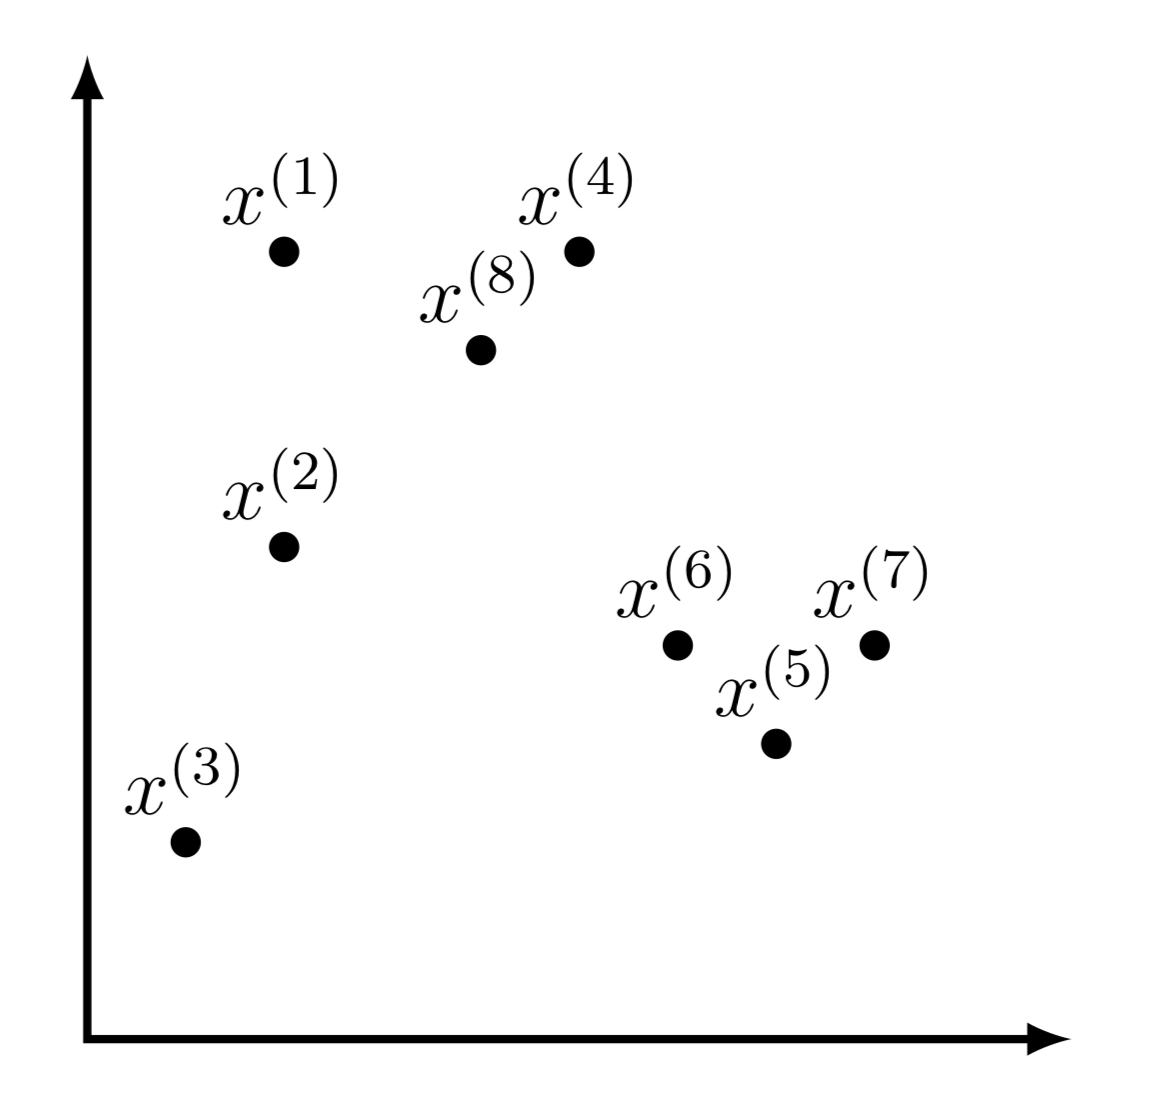
\includegraphics[width=0.4\linewidth]{media/images/kmeans.png}
\caption{Visualisierung des K-Means Datensatzes}
\end{figure}

\begin{subtask}[points=6,title={K-Means Algorithmus}]
Benutzen Sie den K-Means Algorithmus mit der Euklidischen Distanz um diese $8$ Datenpunkte in $K=3$ Cluster einzuteilen.
Nehmen Sie dabei an, dass die Clusterzentren mit den Punkten $x_2$, $x_4$ und $x_8$ initialisiert sind.
Führen Sie zwei Iterationen des K-Means Algorithmus durch und geben Sie die Koordinaten der Zentroide der Cluster an.

\begin{solution}
Wir färben die Cluster ein. Das erste Cluster mit Mittelpunkt $x_2$ ist grün, das zweite Cluster mit Mittelpunkt $x_4$ ist lila und das dritte Cluster mit Mittelpunkt $x_8$ ist blau. Der Abstand zwischen zwei Vektoren $v = (v_1, v_2), u = (u_1, u_2) \in \mathbb{R}^2$ ist gegeben durch $||v-u||= \sqrt{v_1u_1 + v_2u_2}$. Bezeichne $z_i^{(j)}$ das Zentrum des $i$-ten Clusters $(i = 1,2,3)$ im $j$-ten Iterationsschritt. Wir initialisieren $z_1^{(0)} := x_2$, $z_2^{(0)} := x_4$, $z_3^{(0)} := x_8$. Im ersten Schritt berechnen wir \begin{center}
\begin{tabular}{l|rrrrrrrr}
	      & $x_1$ & $x_2$ & $x_3$ & $x_4$ & $x_5$ & $x_6$ & $x_7$ & $x_8$ \\ \hline
	grün: & $3$ & $0$ & $\sqrt{10}$ & $\sqrt{18}$ & $\sqrt{29}$ & $\sqrt{17}$ & $\sqrt{37}$ & $\sqrt{18}$  \\
	lila: & $3$ & $\sqrt{18}$ & $\sqrt{52}$ & $0$ & $\sqrt{29}$ & $\sqrt{17}$ & $5$ & $\sqrt{2}$ \\
	blau: & $\sqrt{5}$ & $\sqrt{8}$ & $\sqrt{34}$ & $\sqrt{2}$ & $5$ & $\sqrt{13}$ & $5$ & $0$
\end{tabular}
\end{center} 
Dabei ist der kl-te Eintrag gegeben durch $||z_k^{(0)}-x_l||$. Durch spaltenweises Vergleichen erhalten wir, dass $x_2$ und $x_3$ grün werden. $x_1, x_5,x_6$ und $x_8$ werden blau und $x_4$ wird lila. Bei $x_7$ haben wir ein Unentschieden zwischen blau und lila. Wir entscheiden uns für blau, da die beiden Nachbarn von $x_7$ ($x_5$ und $x_6$) auch blau sind. Würden wir $x_7$ lila zuordnen, so würden wir die Varianz von lila stark erhöhen, da diese sonst 0 ist. Da der k-means Algorithmus aber die Varianz innerhalb der Cluster minimieren soll, ist blau sicher keine falsche Wahl für $x_7$. \\ Nach dem ersten Iterationsschritt erhalten wir also \begin{align*}
\text{grün}_1 &= \{x_2, x_3\} \text{ mit } z_1^{(1)} = (1,5; 3,5)^T \\
\text{lila}_1 &= \{x_4\} \text{ mit } z_2^{(1)} = x_4 = (5;8)^T \\
\text{blau}_1 &= \{x_1, x_5, x_6, x_7, x_8\} \text{ mit } z_3^{(1)} = (5,4;5,2)^T.
\end{align*}
Für den zweiten Schritt berechnen wir \begin{center}
	\begin{tabular}{l|rrrrrrrr}
		& $x_1$ & $x_2$ & $x_3$ & $x_4$ & $x_5$ & $x_6$ & $x_7$ & $x_8$ \\ \hline
		grün: & $4,53$ & $1,58$ & $1,58$ & $5,70$ & $5,52$ & $4,53$ & $6,52$ & $4,30$  \\
		lila: & $3$ & $4,24$ & $7,21$ & $0$ & $5,39$ & $4,12$ & $5$ & $1,41$ \\
		blau: & $4,4$ & $3,4$ & $5,44$ & $2,82$ & $2,72$ & $1,34$ & $2,86$ & $2,28$
	\end{tabular}
\end{center} 
wobei der kl-te Eintrag durch $||z_k^{(1)}-x_l||$ gegeben ist. Durch spaltenweises Vergleichen erhalten wir (diesmal gibt es kein Unentschieden) \begin{align*}
\text{grün}_2 &= \{x_2, x_3\} \text{ mit } z_1^{(2)} = (1,5; 3,5)^T \\
\text{lila}_2 &= \{x_1, x_4, x_8\} \text{ mit } z_2^{(2)} = x_4 = (3,67;7,67)^T \\
\text{blau}_2 &= \{x_5, x_6, x_7\} \text{ mit } z_3^{(2)} = (7;3,67)^T.
\end{align*}
\end{solution}

\end{subtask}

\end{task}

